%%%%%%%%%%%%%%%%%%%%%%%%%%%%%%%%%
%
%       EXERCÍCIO
%
%%%%%%%%%%%%%%%%%%%%%%%%%%%%%%%%%

\ifdefstring{\atividade}{prova}{%
    \ifdefstring{\modo}{objetivo}{%
        \renewcommand{\valorquestao}{\ValorQObj\ ponto}
    }{%
        \renewcommand{\valorquestao}{\ValorQDisc\ pontos}
    }%
}%

\begin{exercicioBanco}[\valorquestao]
Os gráficos abaixo representam as funções faturamento mensal \(F(x)\) e despesa mensal \(D(x)\) de um pequeno negócio de marmitas, em que \(x\) é o número de marmitas vendidas. Determine o lucro obtido ao vender \(900\) marmitas em um mês, onde lucro é definido pela subtração do faturamento com a despesa.

\begin{center}
    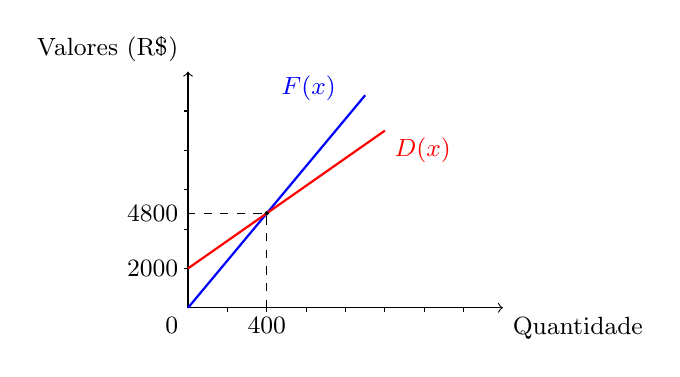
\begin{tikzpicture}[scale=0.5]

        % Eixos
        \draw[->] (0,0) -- (8,0) node[below right] {\small Quantidade};
        \draw[->] (0,0) -- (0,6) node[above left] {\small Valores (R\$)};

        % F(x)
        \draw[domain=0:4.5, smooth, variable=\x, blue, thick] 
            plot ({\x}, {1.2*\x});
        \node[blue, above left] at (4,5) {\small \(F(x)\)};

        % D(x)
        \draw[domain=0:5, smooth, variable=\x, red, thick] 
            plot ({\x}, {0.7*\x + 1});
        \node[red, right] at (5,4) {\small \(D(x)\)};

        % Ponto de interseção (aproximado)
        \filldraw (2,2.4) circle (1.2pt);
        
        \draw[dashed] (2,0) -- (2,2.4) -- (0,2.4);
        \node[below] at (2,0) {\small \(400\)};
        \node[left] at (0,2.4) {\small \(4800\)};
        \node[below left] at (0,0) {\small \(0\)};
        \node[left] at (0,1) {\small \(2000\)};

        % Marcas nos eixos
        \foreach \x in {1,2,3,4,5,6,7}
            \draw (\x,0) -- (\x,-0.1);

        \foreach \y in {1,2,3,4,5}
            \draw (0,\y) -- (-0.1,\y);

    \end{tikzpicture}
\end{center}

% Define as alternativas
\newcommand{\alternativas}{%
    \begin{center}
        \begin{tabularx}{\textwidth}{XXXXX}
            (a) R\$ \(6500{,}00\). &
            (b) R\$ \(6600{,}00\). &
            (c) R\$ \(6700{,}00\). &
            (d) R\$ \(6800{,}00\). &
            (e) R\$ \(6900{,}00\).
        \end{tabularx}
    \end{center}
}

% Resposta correta
\newcommand{\resposta}{A}

% Lógica condicional para exibição
\ifdefstring{\atividade}{lista}{%
    \alternativas
    \vspace{0.5em}
    
    \noindent\textbf{Resposta:} letra \textbf{\resposta}.
}{%
    \ifdefstring{\modo}{objetivo}{%
        \alternativas
    }{%
        % modo = discursiva → não mostra alternativas
    }
}
\end{exercicioBanco}

